%!TEX root = ../thesis.tex
\chapter{基于RGB-D图像的目标检测算法}
\label{chap:detector}
本章主要介绍所提出的两种基于RGB-D图像的目标检测算法3D Faster R-CNN和3D Mask R-CNN。3D Faster R-CNN是在Faster R-CNN\cite{Ren}的基础上,通过引入深度图以解决单从RGB图难以检测缺少纹理物体(Textureless Object)的问题,并且还引入了Spatial Transformer结构使得提取的特征具有旋转不变性。由于3D Faster R-CNN目标检测的结果是框出目标的Bounding Box,因此使得一些框住细长目标的Bounding Box内大部分像素并不属于该目标,这就使得后面的点云匹配算法难以得到满意的结果。因此3D Mask R-CNN根据Mask R-CNN\cite{He2017}对Faster R-CNN的改进思路,对3D Faster R-CNN进行了改进,使得其不仅能得到目标的Bounding Box,还能得到目标的Mask(可以知道Bounding Box内属于检测目标的像素),大大减少了后续匹配算法的难度。

\section{3D Faster R-CNN}
相比于Faster R-CNN,本文所提出的3D Faster R-CNN主要增加对深度信息的处理和Spatial Transformer,分别用于解决Faster R-CNN在实际应用时所不能解决的问题:
\begin{itemize}
\item 难以检测出缺少纹理的物体
\item 对物体的旋转敏感,提取的特征不具有旋转不变性
\end{itemize}

对于缺少纹理的物体,单从RGB图中很难检测出目标,这是一个很显然的问题,但是现在我们可以从对偶RGB-D相机中获取深度图,对于纹理少的物体,可以从深度图中提取特征检测出目标,所以现在的关键问题是如何从深度图中提取特征,并结合到Faster R-CNN中,本文所提出的方法是将深度图转换到HHA,然后再使用CNN提取特征,具体后文会详细介绍。

Faster R-CNN对于物体旋转敏感的问题,归根到底是因为CNN所提取的特征不具有旋转不变性,实际出现这种问题的情况,如图\ref{fig:cat}所示,
\begin{figure}[!ht]
  \centering
  \subfloat[检测旋转前的图片]{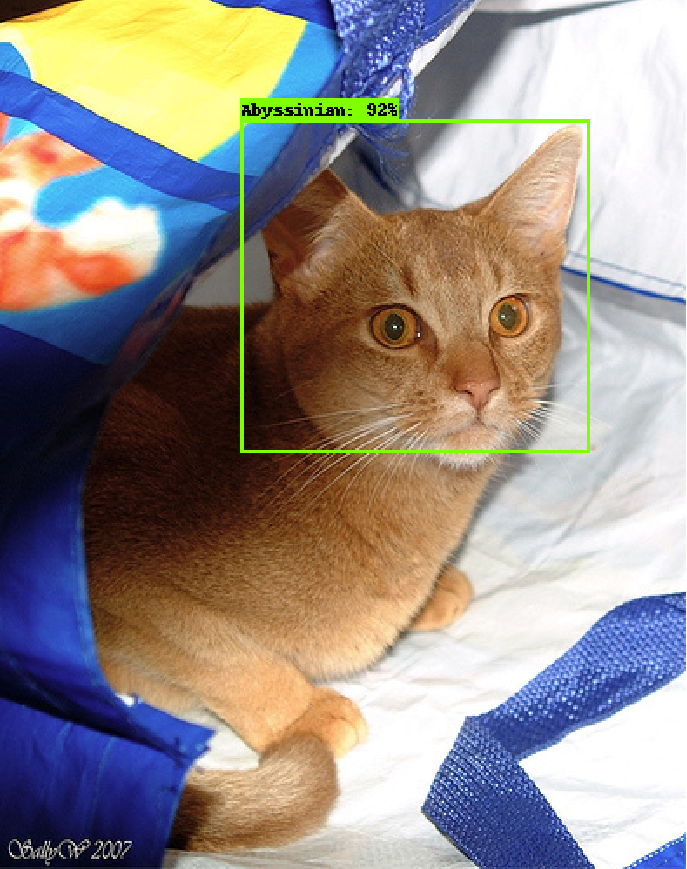
\includegraphics[width=4cm]{cat_up}}
  \hskip1em
  \subfloat[检测旋转后的图片]{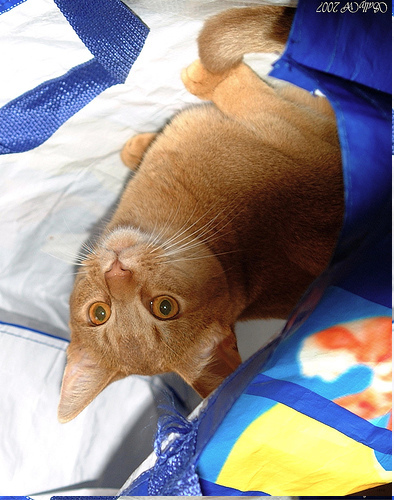
\includegraphics[width=4cm]{cat_down}}
  \caption{Faster R-CNN检测识别宠物猫示例}
  \label{fig:cat}
\end{figure}
其中图(b)只是将图(a)旋转了180度,由于CNN所提取的特征不具有旋转不变性,并且训练所实验的图片中的宠物都是头朝上的,即使图(a)在训练集中,将其旋转180度后,也无法从中检测出目标来。解决这个问题有两个思路:
\begin{itemize}
\item Data Augmentation
\item Spatial Transformer
\end{itemize}
Data Augmentation是通过对训练集中的图片进行旋转以获取不同角度的图片,通过这种方式增大数据集从而使得最终训练得到的模型对各种角度的图片都能识别;Spatial Transformer是一种特殊的网络结构,本文所使用的就这种方式,后文会详细介绍。

\subsection{HHA}

\subsection{Faster RCNN}

\subsection{Spatial Transformer}


\section{3D Mask RCNN}

\section{目标检测实验}

\section{本章小结}

